\documentclass[dc]{svjour}
\usepackage{latexsym}
\usepackage[fleqn]{amstex}
\usepackage{graphics}
%\usepackage{script}
%\usepackage{mytimes}
%\usepackage{mymathtimes}
\usepackage{graphicx}
\usepackage{psfig}
\makeatletter
\@mathmargin\z@
\makeatother
%
%\input{totalin.dc}
%
%\idline{Distrib. Comput (1997) 10: 65--78}{65}
\begin{document}

\def\bsub#1{\def\theequation{#1\alph{equation}}\setcounter{equation}{0}}
\def\esub#1{\def\theequation{\arabic{equation}}\setcounter{equation}{#1}}

\title{Local coupling of shell models\thanks{see also paper by
Claudia Schiffer, Valeria Mazza, Cindy
Crawford, Naomi Campbell, Helena Christensen, Elle McPherson, Eva
Herzigova, Kathy Ireland, Kate Moss, Stephanie Seymour}
 leads to anomalous scaling}

\subtitle{This is a sample article for Distributed Computing}

\author{C. Uhlig\inst{1} \and J. Eggers\thanks{Professor emeritus}\and
I.~Abt\inst{1} \and T.~Ahmed\inst{2} \and
V.~Andreev\inst{3}\and B.~Andrieu\inst{4}\and R.-D. Appuhn
\inst{5}}

\mail{Springer-Verlag}

\institute{Fachbereich Physik, Universit\"at -- Gesamthochschule --
Essen, D-45117 Essen, Germany\and
I. Physikalisches Institut der RWTH, Aachen, Germany\thanks{Supported by
the Bundesministerium f\"ur Forschung und Technologie, FRG under
contract numbers 6AC17P, 6AC47P, 6DO57I, 6HH17P, 6HH27I, 6HD17I, 6HD27I,
6KI17P, 6MP17I, and 6WT87P} \and
III. Physikalisches Institut der RWTH,
Aachen, Germany \and School of Physics and Space Research,
University of Birmingham, Birmingham, UK\thanks{Supported by the UK
Science and Engineering Research Council}
\and Inter-University
Institute for High Energies ULB-VUB, Brussels, Belgium\thanks{Supported
by IISN-IIKW, NATO CRG-890478} \and Rutherford Appleton Laboratory,
Chilton, Didcot, UK \and Institute for Nuclear Physics,
Cracow, Poland\thanks{Supported by the Polish State Committee for
Scientific Research, grant No. 204209101}
\and Physics Department and
IIRPA, University of California, Davis, California,
USA}


%\date{Received: 14 November 1996 / Revised version: 2 January 1997}


\maketitle

\begin{abstract}
This article demonstrates (almost) all possibilities offered by the
new document class \verb|SVJour| in connection with the journal specific
class option \verb|[dc]|. For detailed instructions please consult the
accompanying documentation.
\keywords{Routing schemes -- Universal routing schemes --
Implementation}\end{abstract}

%%%%%%%%%%%%%%%%%
% Introduction  %
%%%%%%%%%%%%%%%%%

\section{Introduction}
\label{sec:intro}

Much of our intuitive understanding of turbulence is based on the
concept of interactions which are local in k-space. Physically,
it is based on the notion that most of the distortion of a turbulence
element or eddy can only come from eddies of comparable size.
Turbulent features which are much larger only uniformly translate
smaller eddies, which does not contribute to the energy transfer.
This immediately leads to the idea of a chain of turbulence elements,
through which energy is transported to the energy dissipating
scales. Accepting such a cascade structure of the turbulent velocity
field, it is natural to assume that the statistical average
of velocity differences ${\bf \delta v(r) = v(x+r) - v(x)}$ over a distance
$|{\bf r}|$ follows scaling laws
\begin{equation}
  \label{vscaling}
     D^{(p)}(r) \equiv \left<|{\bf v(x+r) - v(x)}|^p\right> \sim
r^{\zeta_p}
\end{equation}
in the limit of high Reynolds numbers. By taking velocity {\it differences}
over a distance $r$, one probes objects of corresponding size.

\begin{claim}
This is a claim. Claims are unnumbered and the appearance is exactly the
same as is proofs.
\end{claim}

\begin{proof}
This is a proof. Proofs are unnumbered and the appearance is exactly the
same as is claims.
\end{proof}

\begin{case}\label{romadur}
This is a case. Cases are unnumbered and the appearance is exactly the
same as is claims.
\end{case}

In Case \ref{romadur} you want a different numbering system for your
theorem like environments please see Sect. 2 of the documentation of the
general Springer journals document class.

\begin{remark}
This is a remark. Remarks are unnumbered and the appearance is exactly the
same as is claims.
\end{remark}

\begin{theorem}
This is a theorem. This environment is automagically numbered  and the
layout should be exactly the same as that of the corollary, the
definition, the lemma, and the proposition.
\end{theorem}

\begin{proposition}
This is a proposition. This environment is automagically numbered  and the
layout should be exactly the same as that of the corollary, the
definition, the lemma, and the theorem. You should try it yourself.
\end{proposition}

\begin{lemma}
This is a lemma. This environment is automagically numbered  and the
layout should be exactly the same as that of the corollary, the
definition, the theorem, and the proposition.
\end{lemma}

\begin{definition}
This is a definition. This environment is automagically numbered  and the
layout should be exactly the same as that of the corollary, the
theorem, the lemma, and the proposition.
\end{definition}

\begin{corollary}
This is a corollary. This environment is automagically numbered  and the
layout should be exactly the same as that of the theorem, the
definition, the lemma, and the proposition.
\end{corollary}

If this is not enough, simply define your own environment according to
Sect. 5.2 of the documentation of the general Springer journals document class.

\begin{exercise}
This is an exercise. This environment is automagically numbered  and the
layout should be exactly the same as that of the problem and solution.
\end{exercise}

\begin{problem}
This is an problem. This environment is automagically numbered  and the
layout should be exactly the same as that of the exercise and solution.
\end{problem}

\begin{solution}
This is an solution. This environment is automagically numbered  and the
layout should be exactly the same as that of the problem and exercise.
\end{solution}

\begin{conjecture}
This is an conjecture. This environment is automagically numbered  and the
layout should be exactly the same as that of the example, note,
property, and question.
\end{conjecture}

\begin{example}
This is an example. This environment is automagically numbered  and the
layout should be exactly the same as that of the conjecture, note,
property, and question.
\end{example}

\begin{property}
This is an property. This environment is automagically numbered  and the
layout should be exactly the same as that of the conjecture, note,
example, and question.
\end{property}

\begin{note}
This is an note. This environment is automagically numbered  and the
layout should be exactly the same as that of the example,
conjecture, property, and question.
\end{note}

\begin{question}
This is an question. This environment is automagically numbered  and the
layout should be exactly the same as that of the example,
conjecture, property, and example.
\end{question}

In addition to this assumption of self-similarity, Kolmogorov
\cite{kolmogorov41} also made the seemingly intuitive assumption that
the local statistics of the velocity field should be {\it independent}
of large-scale flow features, from which it is widely separated in scale.
Because the turbulent state is maintained by a mean energy flux
$\epsilon$, the only local scales available are the length $r$ and
$\epsilon$ itself, which leads to the estimate $\delta v \sim
(\epsilon r)^{1/3}$ or
\begin{equation}
  \label{2/3}
    \zeta^{(class)}_p = p/3 .
\end{equation}
At the same time, one obtains an estimate for the Kolmogorov length
\begin{equation}
  \label{eta}
    \eta = (\nu^3/\epsilon)^{1/4}
\end{equation}
where viscosity is important. However, it was only appreciated later
\cite{landau59} that in turbulence long-range correlations
always exist in spite of local coupling. Namely, large-scale fluctuations
of the velocity field will result in a fluctuating energy transfer,
which drives smaller scales. As a result, the statistics of the small-scale
velocity fluctuations will be influenced by the energy transfer
and fluctuations on widely separated scales are correlated,
violating the fundamental assumption implicit in (\ref{2/3}) and
(\ref{eta}).

\begin{itemize}
\item This is the first entry in this list.
\item This is the second entry in this list.
\item This is the third entry in this list.
\item This is the fourth entry in the top level of this list.
\begin{itemize}
\item This is the first entry of the second level in this list.
\item This is the second entry of the second level in this list.
\begin{itemize}
\item This is the first entry of the third level in this list.
\item This is the third entry of the second level in this list.
\item This is the third entry of the third level in this list.
\end{itemize}
\item This is the third entry of the second level in this list.
\end{itemize}
\item This is the fifth entry in this list.
\item This is the last entry in this list.
\end{itemize}

Indeed, Kolmogorov \cite{kolmogorov62} and Obukhov \cite{obukhov62}
later proposed the existence of
corrections to the scaling exponents (\ref{2/3}),
\begin{equation}
  \label{correct}
     \zeta_p = p/3 + \delta\zeta_p \;, \delta\zeta_p \ne 0
\end{equation}
which were subsequently confirmed experimentally
%[5--8].
\cite{anselmet84,benzi93a,benzi93b,herweijer95}.
On one hand, careful laboratory
experiments have been performed at ever higher Reynolds numbers
\cite{anselmet84,castaing90}. On the other hand, a new method of
data analysis \cite{benzi93a,benzi93b} has been successful
in eliminating part of the effects of viscosity.
\begin{enumerate}
\item This is the first entry in this numbered list.
\item This is the second entry in this numbered list.
\item This is the third entry in this numbered list.
\item This is the fourth entry in the top level of this numbered list.
\begin{enumerate}
\item This is the first entry of the second level in this numbered list.
\item This is the second entry of the second level in this numbered list.
\begin{enumerate}
\item This is the first entry of the third level in this numbered list.
\item This is the third entry of the second level in this numbered list.
\item This is the third entry of the third level in this numbered list.
\end{enumerate}
\item This is the third entry of the second level in this numbered list.
\end{enumerate}
\item This is the fifth entry in this numbered list.
\item This is the last entry in this numbered list.
\end{enumerate}
In particular,
for the highest moments up to $p = 18$ significant corrections to
classical scaling were found, a currently accepted value for the so-called
intermittency parameter $\mu$ being
\cite{anselmet84}
\begin{equation}
  \label{mu}
     \mu = -\delta\zeta_6 = 0.2 ,
\end{equation}
which is a 10 \% correction. The existence of corrections like
(\ref{mu}) implies that on small scales large fluctuations are much more
likely to occur than predicted by classical theory.

This ``intermittent'' behavior is thus most noticeable in derivatives
of the velocity field such as the local rate of energy dissipation
\[
\epsilon({\bf x},t) = \frac{\nu}{2}\left(\partial u_i/\partial x_k
             + \partial u_k/\partial x_i\right)^2 .
\]
Much of the research in turbulence has been devoted to the study
of the spatial structure of $\epsilon({\bf x},t)$
\cite{kolmogorov62,nelkin89}, but which will not be considered here.
The statistical average of this quantity is what we simply called
$\epsilon$ before. Owing to energy conservation, it must be equal
to the mean energy transfer.

The local coupling structure of turbulence has inspired the study
of so-called shell models, where each octave in wavenumber is
represented by a {\it constant} number of modes, which are
only locally coupled. This allows to focus on the implications of
local coupling for intermittent fluctuations, disregarding
effects of convection and mixing. The mode representation
of a single shell serves as a simple model for the ``coherent
structures'' a turbulent velocity field is composed of, and which
to date have only been poorly characterized, both experimentally and
theoretically.


%%%%%%%%%%%%%%%%%
% section 2     %
%%%%%%%%%%%%%%%%%

\section{Two cascade models}
\label{sec:model}
\subsection{Reduced wave vector set approximation}
\subsubsection{Test for heading of third order}
\paragraph{The REWA model.}
The REWA model
\cite{eggers91a,grossmann94a} is based on the full Fourier-transformed
Navier-Stokes equation within a volume of periodicity $(2\pi L)^{3}$. In order
to restrict the excited Fourier-modes of the turbulent velocity field
to a numerically tractable number, the Navier-Stokes equation is
projected
onto a self-similar set of wave vectors ${\cal K}=\bigcup_{\ell}{\cal
  K}_{\ell}$. Each of the wave vector shells ${\cal K}_{\ell}$ represents
an octave of wave numbers. The shell ${\cal K}_{0}$ describes
the turbulent
motion of the large eddies which are of the order of the outer length scale
$L$. This shell is defined by $N$ wave vectors ${\bf k}^{(0)}_{i}$: ${\cal
  K}_{0}=\{{\bf k}^{(0)}_{i}:i=1,\dots,N\}$.  Starting with the generating
shell ${\cal K}_{0}$, the other shells ${\cal K}_{\ell}$ are found by a
successive rescaling of ${\cal K}_{0}$ with a scaling factor 2: ${\cal
  K}_{\ell}=2^{\ell} {\cal K}_{0}$. Thus each ${\cal K}_{\ell}$
consists of the $N$ scaled wave vectors $ 2^{\ell}{\bf k}_{i}^{(0)},\
i=1,\dots,N$. The shell ${\cal K}_{\ell}$ represents eddies at length scales
$r\sim 2^{-\ell}L$, i.e. to smaller and smaller eddies as the shell index
$\ell$ increases.
At scales $r \approx \eta$ the fluid motion is damped by
viscosity $\nu$, thus preventing the generation of infinitely
small scales. Hence we only need to simulate shells ${\cal K}_{\ell},
\ell < \ell_{\nu}$, where $\ell_{\nu} \approx \log_2(L/\eta)$
is chosen such that the amplitudes in ${\cal K}_{\ell_{\nu}}$ are
effectively zero. In this representation the Navier-Stokes equation for
incompressible fluids reads for all ${\bf k}\in {\cal
  K}=\bigcup_{\ell=0}^{\ell_{\nu}}{\cal K}_{\ell}$:
\bsub{7}
  \begin{eqnarray}
  \label{incompNSeq}
    \frac{\partial}{\partial t}u_{i}({\bf k},t)&=&
       -\imath M_{ijk}({\bf k})\sum_{
      {\bf p},{\bf q}\in{\cal K}\atop {\bf k}={\bf p}+{\bf q}} u_{j}({\bf
      p},t)u_{k}({\bf q},t)\nonumber\\ &&
      -\nu k^{2}u_{i}({\bf k},t)+f_{i}({\bf
      k},t)\label{NSeq}\\
    {\bf k}\cdot {\bf u}({\bf k},t)&=&0\label{compress} .
  \end{eqnarray}
\esub{7}%
The coupling tensor $M_{ijk}({\bf k})=\left[k_{j}P_{ik}({\bf
  k})+k_{k}P_{ij}({\bf k})\right]/2$ with the projector $P_{ik}({\bf
  k})=\delta_{ik}-k_{i}k_{k}/k^{2}$ is symmetric in $j,k$ and $M_{ijk}({\bf
  k})=-M_{ijk}(-{\bf k})$. The inertial part of (\ref{NSeq}) consists
of all triadic interactions between modes with ${\bf k}={\bf p}+{\bf q}$.
They are the same as in the full Navier-Stokes equation for this triad.
The velocity field is driven by an external force ${\bf f}({\bf
  k},t)$ which simulates the energy input through a large-scale instability.

%\begin{figure*}\sidecaption
%\psfig{figure=fig1.eps,width=6.7cm}
%\resizebox{0.3\hsize}{!}{\includegraphics*{fig1.eps}}
%    \caption{A two-dimensional projection of the $k$-vectors
%    in shell ${\cal K}_0$ for both the REWA models considered here.
%    The small set ($\times$) contains all vectors with -1, 0, and 1 as
%    components. The large set ($\bigcirc$), in addition, contains
%    combinations with $\pm1/2$ and $\pm 2$
%    }
%  \label{fig:sets}
%\end{figure*}

Within this approximation scheme the energy of a shell is
\begin{equation}
  \label{energy}
  E_{\ell}(t)=\frac{1}{2}\sum_{{\bf k}\in{\cal K}_{\ell}} |{\bf u}({\bf
    k},t)|^{2},
\end{equation}
and in the  absence of any viscous or external driving the
total energy of the flow field
$E_{tot}(t)=\sum_{\ell=0}^{\ell_{\nu}} E_{\ell}(t)$ is conserved.
The choice of generating wave vectors ${\bf k}^{(0)}_i$ determines
the possible triad interactions. This choice must at least guarantee
energy transfer between shells and some mixing within a shell. In
\cite{eggers91a,grossmann94a} different choices for
wavenumber sets ${\cal K}_0$ are investigated. The larger the number
$N$ of wave numbers, the more effective the energy transfer. Usually
one selects directions in ${\bf k}$-space to be distributed evenly
over a sphere. However, there are different possibilities which
change the relative importance of intra-shell versus inter-shell
couplings. In this paper, we are going to investigate two different
wave vector sets, with $N=26$ and $N=74$, which we call the small and the
large wave vector set, respectively. In Fig.~1 a two-dimensional
projection of both sets is plotted. The large wave vector set also
contains some next-to-nearest neighbor interactions between shells,
which we put to zero here, since they contribute little to the
energy transfer. The small set allows 120 different interacting triads,
the large set 501 triads, 333 of which are between shells.

\begin{figure}%f2
%\psfig{figure=fig2.eps,width=3.25cm}
\sidecaption
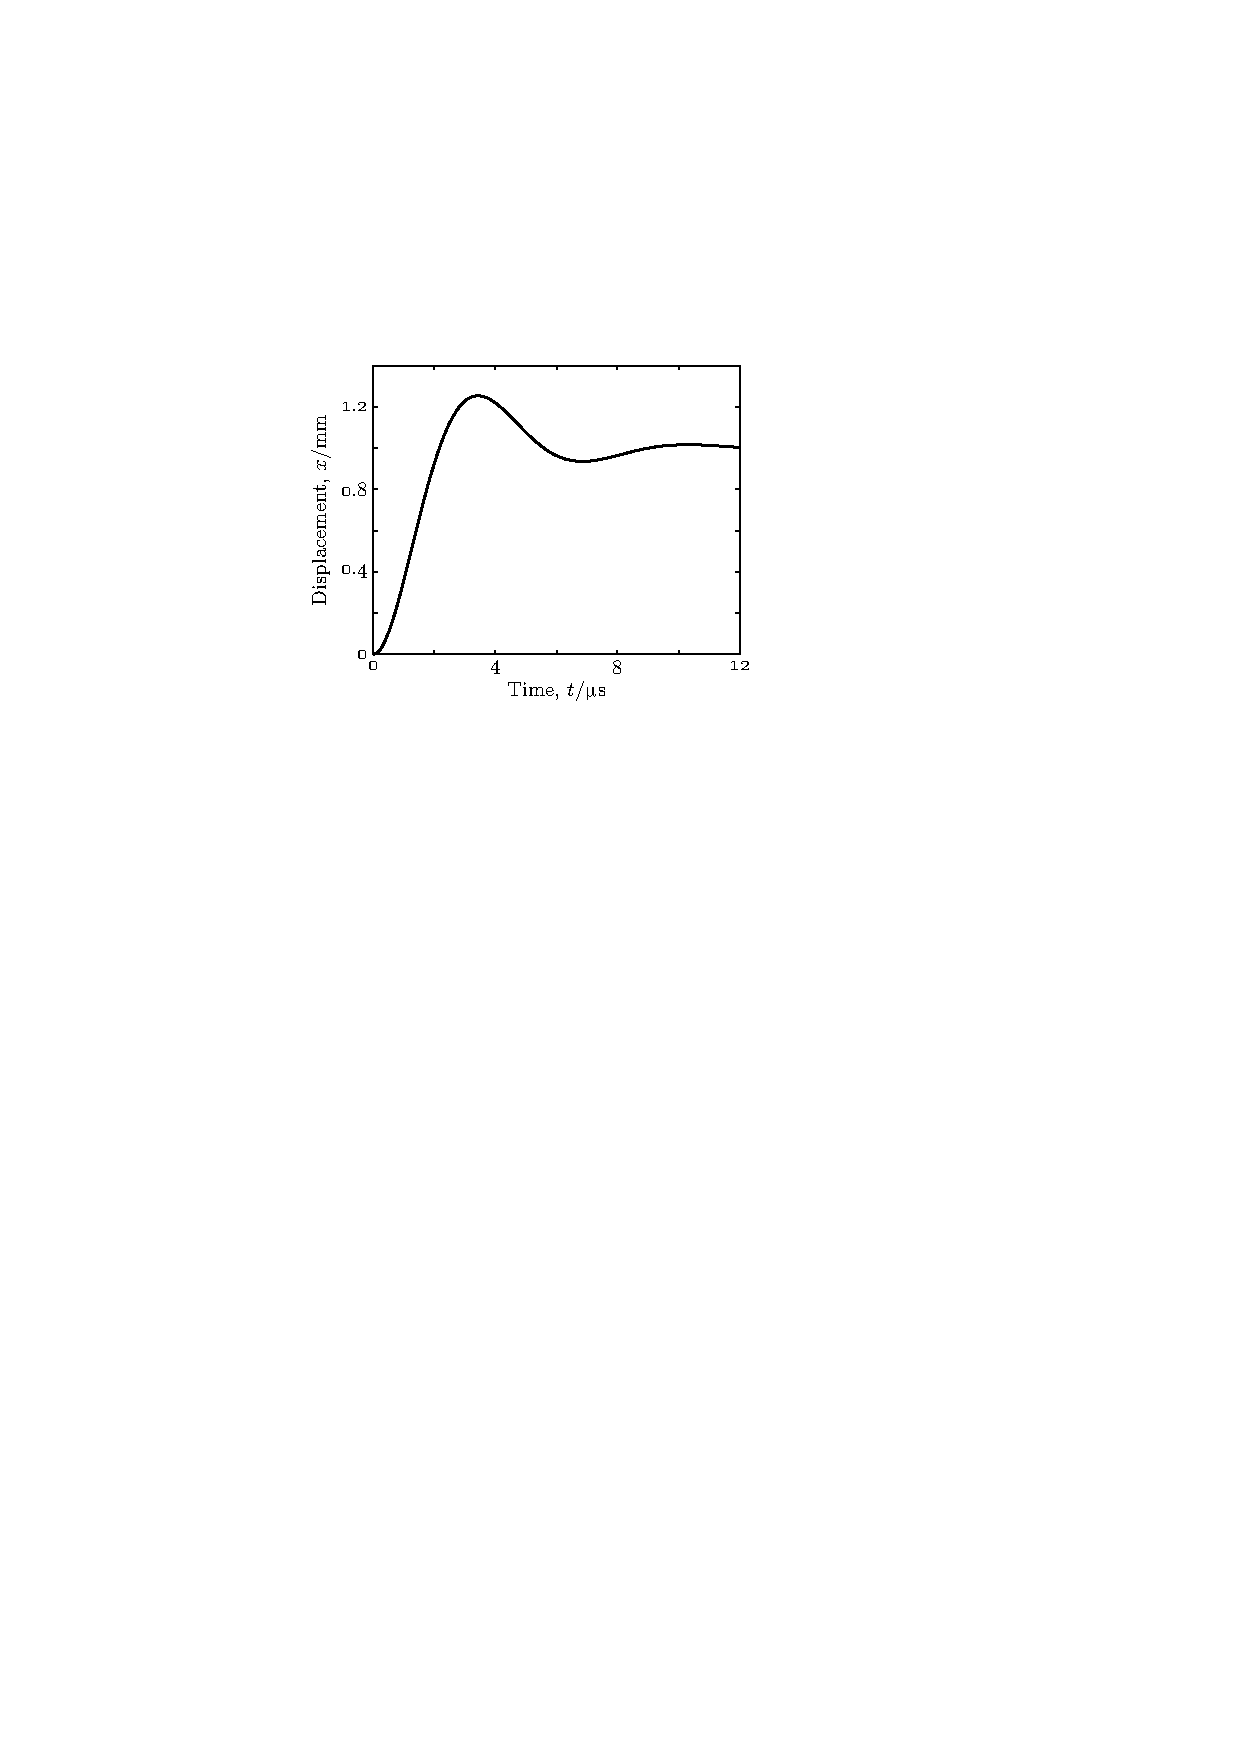
\includegraphics[width=2cm,bb=0 0 192 635]{fig2}
  \caption{The structure of a local cascade.
    Eddies of size $r\sim 2^{-\ell}L$ are
    represented by their total energy $E_{\ell}$.
    Only modes of
    neighboring shells interact, leading to a local energy
    transfer $T_{\ell\rightarrow\ell+1}(t)$. The cascade is driven by
    injecting energy into the largest scale with rate
    $T_{0}^{(in)}(t)$. The turbulent motion is damped by viscous dissipation
    at a rate
    $T_{\ell}^{(diss)}(t)$
    }
  \label{fig:modelstructure}
\end{figure}

Since in the models we consider energy transfer is purely local,
the shell energies $E_{\ell}(t),\ \ell=0,\dots,\ell_{\nu}$ only change
in response to energy influx $T_{\ell-1\rightarrow \ell}$ from above
and energy outflux $T_{\ell\rightarrow \ell+1}$ to the lower
shell. In addition, there is a rate of viscous dissipation
$T_{\ell}^{(diss)}(t)$ which is concentrated on small scales,
and a rate of energy input $T_{0}^{in}(t)$, which feeds
the top level only, cf. Fig.~\ref{fig:modelstructure}.

From (\ref{NSeq}) we find an energy balance equation which governs
the time evolution of the shell energies $E_{\ell}(t)$
\begin{multline}
  \label{energyconservationlaw}
  \frac{d}{dt} E_{\ell}(t)=T_{\ell-1\rightarrow \ell}(t)-T_{\ell\rightarrow
    \ell+1}(t)+T_{\ell}^{(diss)}(t)+\\ T_{0}^{(in)}(t)\delta_{\ell0} .
\end{multline}
The different transfer terms are found to be
\bsub{10}
\begin{align}
\label{FWtransfer}
  T_{\ell\rightarrow \ell+1}(t) &=
       2\imath \sum_{\triangle^{(\ell+1)}_{(\ell)}}
  M_{ijk}({\bf k}) u_{i}^{*}({\bf k},t)u_{j}({\bf p},t)u_{k}({\bf q},t)
  \label{FWta}\\
  T_{0}^{(in)}(t) &= \sum_{{\bf k}\in{\cal K}_{0}} \mbox{\rm Re}\left({\bf
    u}^{*}({\bf k},t)\cdot{\bf f}({\bf k},t)\right) \label{FWtb}\\
  T_{\ell}^{(diss)}(t) &= -\nu \sum_{{\bf k}\in{\cal K}_{\ell}} k^{2}|{\bf
    u}({\bf k},t)|^{2} \label{FWtc}.
\end{align}
\esub{10}%
In (\ref{FWta}) $\sum_{\triangle^{(\ell+1)}_{(\ell)}}$
indicates the summation over all
next-neighbor triads ${\bf k}={\bf p}+{\bf q}$ with ${\bf k}\in {\cal
  K}_{\ell},\ {\bf p}\in{\cal K}_{\ell+1}$ and ${\bf q}\in{\cal
  K}_{\ell}\bigcup{\cal K}_{\ell+1}$.

The driving force ${\bf f}({\bf k},t)$ is assumed to act only on the
largest scales, and controls the rate of energy input
$T_{0}^{(in)}(t)$. As in \cite{eggers91a}
we choose ${\bf f}({\bf k},t)$ to ensure constant energy input
$T^{(in)}_0 = \epsilon$ :

\bsub{11}
    \begin{eqnarray}
    \label{force}
      {\bf f}({\bf k},t)&=&\frac{\epsilon {\bf u}({\bf k},t)}{N|{\bf
          u}({\bf k},t)|^{2}} \enspace \mbox{for all } {\bf k}\in{\cal
        K}_0\\ {\bf f}({\bf k},t)&=&0 \enspace \mbox{for all } {\bf
        k}\not\in{\cal K}_0 .
    \end{eqnarray}
\esub{11}%

\begin{equation}
  \label{re}
    Re = \frac{L U}{\nu} = \frac{\epsilon L^2}{\left< E_0 \right>\nu} ,
\end{equation}

\begin{figure*}%f3
\sidecaption
\resizebox{10cm}{!}{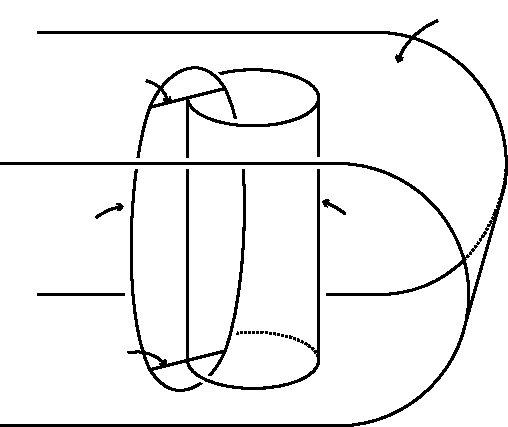
\includegraphics{fig3.eps}}
  \caption{Log-log-plot of the structure function
    $\tilde{D}_{\ell}^{(2)}=\left<E_{\ell}\right>$ versus level number
    for the small cascade. At large scales, where the influence of
    dissipation is negligible, classical scaling is observed.
    At small scales the
    turbulent motion is damped by viscosity.
    The Reynolds number is $Re = 4.2\cdot10^5$
    }
  \label{fig:scaling}
\end{figure*}

This leads to a
stationary cascade whose statistical properties are governed by the
complicated chaotic dynamics of the nonlinear mode interactions.
Owing to energy conservation, viscous dissipation equals the energy
input on average. The Reynolds number is given by
since $T = \left<E_0\right> / \epsilon$ sets a typical turnover
time scale of the energy on the highest level. We believe
$T$ to be of particular relevance, since the large-scale fluctuations
of the energy will turn out to be responsible for the intermittent
behavior we are interested in. In \cite{grossmann94a}, for example,
time is measured in units of $L^{2/3} \epsilon^{-1/3}$, which
typically comes out to be 1/10th of the turnover time of the energy $T$.
As we are going to see below, this is rather a measure
of the turnover times of the individual Fourier modes.
Figure \ref{fig:scaling} shows the scaling of the mean energy
in a log-log plot at a Reynolds number of $4.2 \cdot 10^5$.
The inertial range extends over three decades, where a power
law very close to the prediction of classical scaling is seen.
Below the 10th level the energies drop sharply due to viscous
dissipation. In Sect.~3 we are going to turn
our attention to the small corrections to 2/3-scaling, hardly
visible in Fig.~\ref{fig:scaling}. Still, there are considerable
fluctuations in this model, as evidenced by the plot of the energy
transfer in Fig.~\ref{fig:scaling}. Typical excursions from the
average, which is normalized to one, are quite large. Ultimately,
these fluctuations are responsible for the intermittency
corrections we are going to observe.

\begin{figure}%f5
\psfig{figure=fig5.eps,width=6.45cm}
  \caption{Energy of a shell ($\ell=2$) as a function of time.
    The rapid fluctuations come
    from the motion of individual Fourier modes.
    A much longer time scale is revealed by performing a
    floating average over one turnover time of
    the second level (bold line).
    The time is given in units of $T = \left<E_{0}\right>/\epsilon$}
  \label{fig:energy}
\end{figure}

Thus within the REWA-cascade we
are able to numerically analyze the influence of fluctuations
on the stationary statistical properties of a cascade with local energy
transfer on the basis of the Navier-Stokes
equation. In Fig.~\ref{fig:energy} we plot the time evolution
of the energy on the second level of the cascade. One observes
short-scale fluctuations, which result from the motion of individual
Fourier modes within one cascade level. However, performing a floating
average reveals a {\it second} time scale, which is of the same order as the
turnover time of the top level. As we are going to see in
Sect.~4, this disparity of time scales is even
more pronounced on lower levels. The physics idea is the same as
in the microscopic foundation of hydrodynamics,
where conserved quantities are assumed to move on much slower time scales
than individual particles.
This motivates us to consider the energy as the only dynamical variable
of each shell, and to represent the rapid fluctuations of
Fig.~\ref{fig:energy} by a white-noise Langevin force. In this approximation
we still hope to capture the rare, large-scale events characteristic
of intermittent fluctuations, since the conserved
quantity is the ``slow'' variable of the system. Similar ideas have also
been advanced for the conservative dynamics of a non-equilibrium
statistical mechanical system \cite{spohn}.

\subsection{The Langevin-cascade}

In this model we take a phenomenological view of the process of energy
transfer. The chaotic dynamics of the REWA-cascade is modeled by a stochastic
equation. We make sure to include the main physical features of
energy conservation and local coupling. In particular,
the dynamics is simple enough to allow for analytical insight into
the effects of fluctuating energy transfer \cite{eggers94}.

As in the REWA-cascade, the turbulent flow field is
described by a sequence of eddies decaying successively
(Fig.~\ref{fig:modelstructure}). The eddies at
length scales $r\sim 2^{-\ell}L$ are represented by their energy
$E_{\ell}(t)$.
As before we restrict ourselves to local energy transfer,
and thus the time evolution of the
shell energies $E_{\ell}(t)$ is governed by
(\ref{energyconservationlaw}). The crucial step is of course to choose
an appropriate energy transfer $T_{\ell\rightarrow\ell+1}(t)$.
For simplicity, we restrict ourselves to a Langevin process with a white
noise force. Thus the local transfer $T_{\ell\rightarrow \ell+1}(t)$ is
split into a deterministic and a stochastic part $T_{\ell\rightarrow
  \ell+1}(t) = T_{\ell\rightarrow \ell+1}^{(det)}(t)+
T_{\ell\rightarrow\ell+1}^{(stoch)}(t)$ where both
parts should depend only on the local length scale $2^{-\ell}L$ and
the neighboring energies $E_{\ell}$ and $E_{\ell+1}$. The most
general form dimensionally consistent with this has been given in
\cite{eggers94}. For simplicity, here we restrict ourselves to the specific
form
\bsub{13}
  \begin{align}
  \label{Letrans}
    T_{\ell\rightarrow \ell+1}^{(det)}(t)&= D
    \frac{2^{\ell}}{L}\left(E_{\ell}^{3/2}(t)-E_{\ell+1}^{3/2}(t)\right)
    \label{Letransa}\\
    T_{\ell\rightarrow \ell+1}^{(stoch)}(t)&= R
    \left(\frac{2^{(\ell+1)}}{L}\right)^{1/2}
      (E_{\ell}(t)E_{\ell+1}(t))^{5/8}
      \xi_{\ell+1}(t)\label{Letransb}\\
      T_{\ell}^{(in)}(t)&= \epsilon
    \delta_{\ell 0} \label{Letransc}\\
     T^{(diss)}_{\ell}(t) &=
        -\nu(2^{-\ell}L)^{-2} E_{\ell} . \label{Letransd}
  \end{align}
\esub{13}%
The white noise is represented by
$\xi_{\ell}$, i.e. $\left<\xi_{\ell}(t)\right>=0$ and
$\left<\xi_{\ell}(t)\xi_{\ell'}(t')\right>=2\delta_{\ell\ell'}\delta(t-t')$.
We use Ito's \cite{gardiner83} definition in (\ref{Letransb}).
To understand the dimensions appearing in (\ref{Letrans}), note
that $u_{\ell} \sim E_{\ell}^{1/2}$ is a local velocity scale and
$k \sim 2^{\ell}/L$ is a wavenumber. Thus (\ref{Letransa})
dimensionally represents the energy transfer (\ref{FWta}).
In (\ref{Letransb}) the powers are different, since $\xi$ carries
an additional dimension of $1/\mbox{time}^{1/2}$.
It follows from (\ref{Letransa}) that the sign of the deterministic
energy transfer depends on which of the neighboring energies
$E_{\ell}$ or $E_{\ell+1}$ are greater. If for example $E_{\ell}$
is larger, $T^{(det)}_{\ell\rightarrow\ell+1}(t)$ is positive,
depleting $E_{\ell}$ in favor of $E_{\ell+1}$. Hence the
deterministic part tends to equilibrate the energy among the
shells. The stochastic part, on the other hand, is symmetric with
respect to the two levels $\ell$ and $\ell+1$. This reflects
our expectation that in equilibrium it is equally probable for
energy to be scattered up or down the cascade.

The combined effect of (\ref{Letransa}) and (\ref{Letransb}) is
that without driving, energies fluctuate around a common mean value.
This equipartition of energy in equilibrium is precisely
what has been predicted on the basis of the Navier-Stokes
equation \cite{kraichnan73,orszag73}.
The only free parameters appearing in the transfer are thus the
amplitudes $D$ and $R$. If $R$ is put to zero, the motion is
purely deterministic, and one obtains the simple solution
\begin{equation}
  \label{statenerg}
  E_{\ell}^{(0)}=C 2^{-(2/3)\ell}\ \mbox{with}\
           C=\left(\frac{2\epsilon L}{D}\right)^{2/3}.
\end{equation}
This corresponds to a classical Kolmogorov solution with no
fluctuations in the transfer. The amplitude $D$ of the deterministic
part is a measure of the effectiveness of energy transfer. On the other
hand $R$ measures the size of fluctuations. In \cite{eggers94}
it is shown that a finite $R$ necessarily leads to intermittency
corrections in the exponents. In the next section we are going to
determine the model parameters for the two REWA cascades we are
considering.


%%%%%%%%%%%%%%%%%%%
% acknowledgments %
%%%%%%%%%%%%%%%%%%%

\begin{acknowledgement}
We are grateful to R. Graham for useful discussions and to
J. Krug for comments on the manuscript.
This work is supported by the Sonderforschungsbereich 237 (Unordnung und
grosse Fluktuationen).
\end{acknowledgement}


%%%%%%%%%%%%%%%%%
% bibliography  %
%%%%%%%%%%%%%%%%%

\begin{thebibliography}{47}

\bibitem{kolmogorov41} A.~N.~Kolmogorov,
C.~R.~Akad.~Nauk~SSSR {\bf 30},~301 (1941);
C.~R.~Akad.~Nauk~SSSR {\bf 31}, 538 (1941);
C.~R.~Akad.~Nauk~SSSR {\bf 32}, 16 (1941)

\bibitem{landau59} L.~D.~Landau and E.~M.~Lifshitz, {Fluid
    Mechanics} (Pergamon, Oxford, 1959; third edition, 1984)

\bibitem{kolmogorov62} A.~N.~Kolmogorov,  J. Fluid Mech. {\bf 13},
 83 (1962)

\bibitem{obukhov62} A.~M.~Obukhov,  J. Fluid Mech. {\bf
    13}, 77 (1962)

\bibitem{anselmet84} F.~Anselmet, Y.~Gagne, E.~J.~Hopfinger and R.~Antonia,
J. Fluid Mech. {\bf 140}, 63 (1984)

\bibitem{benzi93a} R.~Benzi, S.~Ciliberto, R.~Tripiccione, C.~Baudet,
  F.~Massaioli and S.~Succi,  Phys. Rev. E {\bf 48}, R29 (1993)

\bibitem{benzi93b} R.~Benzi, S.~Ciliberto, C.~Baudet, G.~R.~Chavarria and
  R.~Tripiccione,  Europhys. Lett. {\bf 24}, 275 (1993)

\bibitem{herweijer95} J.~Herweijer and W.~van~de~Water,  Phys.
    Rev. Lett. {\bf 74}, 4651 (1995)

\bibitem{castaing90} B.~Castaing, Y.~Gagne and E.~J.~Hopfinger,
 Physica D {\bf 46}, 177 (1990)

\bibitem{nelkin89} M.~Nelkin, J. Stat. Phys. {\bf 54}, 1 (1989)

\bibitem{douady91} S.~Douady, Y.~Couder, and M.~E.~Brachet,
 Phys. Rev. Lett. {\bf 67}, 983 (1991)

\bibitem{kida92} S.~Kida and K.~Ohkitany,  Phys. Fluids A
         {\bf 4}, 1018 (1992)

\bibitem{moffatt94} H.~K.~Moffatt, S.~Kida, and K.~Ohkitany,
        {J. Fluid Mech.} {\bf 259}, 241 (1994)

\bibitem{jimenez93} J.~Jim\'{e}nez, A.~A.~Wray, P.~G.~Saffman, and
        R.~S.~Rogallo,  J. Fluid Mech. {\bf 255}, 65 (1993)

\bibitem{she94} Z.-S.~She and E.~Leveque,  Phys. Rev. Lett.
    {\bf 72}, 336 (1994)

\bibitem{lvov95} V.~L'vov and I.~Procaccia,
  Phys. Rev. E {\bf 52}, 3840 (1995);
 Phys. Rev. E {\bf 52}, 3858 (1995)

\bibitem{eggers91a} J.~Eggers and S.~Grossmann,  Phys. Fluids A
    {\bf 3}, 1958 (1991)

\bibitem{grossmann94a} S.~Grossmann and D.~Lohse,  Phys. Fluids
    {\bf 6}, 611 (1994)

\bibitem{eggers92} J.~Eggers,  Phys. Rev. A {\bf 46}, 1951 (1992)

\bibitem{eggers94} J.~Eggers,  Phys. Rev. E {\bf 50}, 285 (1994)

\bibitem{domaradzki95} J.~A.~Domaradzki and W.~Liu,  Phys. Fluids {\bf 7}, 2025 (1995)

\bibitem{obukhov71} A.~M.~Obukhov,  Atmos. Ocean. Phys.
 {\bf 7}, 471 (1971)

\bibitem{gledzer73} E.~B.~Gledzer,  Sov. Phys. Dokl.
 {\bf 18}, 216 (1973)

\bibitem{yamada87} M.~Yamada and K.~Ohkitami, J. Phys. Soc. Jpn
  {\bf 56}, 4210 (1987)

\bibitem{grossmann93} S.~Grossmann and D.~Lohse,  Europhys. Lett. {\bf 21}, 201 (1993)

\bibitem{glr96} S.~Grossmann, D.~Lohse, and A. Reeh,
Phys. Rev. Lett. {\bf 77}, 5369 (1996)

\bibitem{eggers91b} J.~Eggers and S.~Grossmann,  Phys. Lett. A
{\bf 156}, 444 (1991)

\bibitem{farge92} M.~Farge,  Ann. Rev. Fluid Mech. {\bf 24},
               395 (1992)

\bibitem{meneveau91} C.~Meneveau, J. Fluid Mech. {\bf 232},
              469 (1991)

\bibitem{spohn} P.~L.~Garrido, J.~L.~Lebowitz, C.~Maes, and
H.~Spohn, Physical Rev. A {\bf 42}, 1954 (1990)

\bibitem{gardiner83} C.~W.~Gardiner, {Handbook of Stochastic Methods}
(Springer, Berlin, 1983)

\bibitem{kraichnan73} R.~H.~Kraichnan,  J. Fluid Mech. {\bf 59}, 745 (1973)

\bibitem{orszag73} S.~Orszag, ``Lectures on the Statistical
     Theory of Turbulence'' in: {Fluid Dynamics 1973, Les
    Houches Summer School of Theoretical Physics}, edited by R.~Balian and
    J.~L.~Peube (Gordon and Breach, 1977)

\bibitem{tennekes80} H.~Tennekes and J.~L.~Lumley, {A First Course in
    Turbulence} (MIT Press, 6th ed., 1980)

\bibitem{grossmann92} S.~Grossmann and D.~Lohse,  Z. Phys. B {\bf 89}, 11 (1992)

\bibitem{press92} W.~H.~Press, S.~A.~Teukolsky, W.~T.~Vetterling,
  and B.~P.~Flannery, {Numerical Recipes} (Cambridge University
       Press, 2nd edition, 1986)

\bibitem{kerr78} R.~M.~Kerr and E.~D.~Siggia,  J. Stat. Phys. {\bf 19}, 543 (1978)

\bibitem{yeung89} P.~K.~Yeung and S.~B.~Pope,
J. Fluid Mech. {\bf 207}, 531 (1989)

\bibitem{kraichnan74} R.~H.~Kraichnan,  J. Fluid Mech. {\bf 62}, 305 (1974)

\bibitem{uhlig96} C.~Uhlig and J.~Eggers,  Z. Phys. B, to be published
                  (1997)

\bibitem{majda90} A.~J.~Majda,  SIAM Review {\bf 33}, 349 (1990)

\bibitem{olla95} P.~Olla,
Phys. Fluids {\bf 7}, 1598 (1995)

\bibitem{uhlig94} C.~Uhlig and J.~Eggers,  {unpublished
                  manuscript} (1994)

\bibitem{Siggia77} E.~D.~Siggia,  Phys. Rev. A {\bf 15}, 1730 (1977)


\bibitem{jensen91} M.~H.~Jensen, G.~Paladin, and A.~Vulpiani,
Phys. Rev. A  {\bf 43}, 798 (1991)

\bibitem{benzi95} R.~Benzi et al,  Phys. Fluids {\bf 7}, 617 (1995)

\bibitem{benzi93c} R.~Benzi, L.~Biferale, and G.~Parisi, Physica D {\bf 65}, 163 (1993)

\end{thebibliography}
\vspace*{4mm}
\begin{biography}
{Son Pham}
is currently a professor of Computer
Science, College of Engineering and Computer Science at the California
State University at Northridge. His research interests include Computer
Graphics and Software Engineering. He has published a dozen refereed
academic/technical papers in Computer Science. He is a member of ACM.
Pham received his BA in Mathematics from the University of Saigon,
VietNam in 1973; MA in Mathematics from University of Louisville,
Kentucky in 1975; Ph.D. in Statistics from the University of Cincinnati,
Ohio in 1978; and PD in Computer Science from the University of
California, Berkeley in 1980.
\end{biography}
\newpage
\begin{biography}
{Mel Slater}
joined the Department of Computer Science,
Queen Mary and Westfield College (University of London) in 1981. Since
1982 he has been involved in teaching and research in computer graphics.
He produced an early implementation of the GKS graphics standard, and
was involved in the ISO graphics group, with responsibility for the
PASCAL language binding to GKS. He co-authored an undergraduate textbook
on computer graphics, which was published in 1987. He is a principal
investigator in several funded research projects, in particular the
European Community ESPRIT funded SPIRIT Workstation project, and a
project on Virtual Reality with the London Parallel Applications Centre.
He was visiting professor in the Computer Science Division of Electrical
Engineering and Computer Sciences, University of California at Berkeley
in the spring semesters 1991 and 1992.
\end{biography}

\begin{biography}{W. Kenneth Stewart} is an assistant scientist at the
Deep Submergence Laboratory of the Woods Hole Oceanographic Institution.
His research interests include underwater robotics, autonomous vehicles
and smart ROVs, multisensor modeling, real-time acoustic and optical
imaging, and precision underwater surveying. Stewart has been going to
sea on oceanographic research vessels for 19 years, has developed
acoustic sensors and remotely-operated vehicles for 6000-m depths, and
has made several deep dives in manned submersibles, including a 4000-m
excursion to the {\it USS Titanic} in 1986. He is a member of the Marine
Technology Society, Oceanography Society, IEEE Computer Society, ACM
SIGGRAPH, and NCGA. Stewart received a PhD in oceanographic engineering
from the Massachusetts Institute of Technology and Woods Hole
Oceanographic Institution Joint Program in 1988, a BS in ocean
engineering from Florida Atlantic University in 1982, and an AAS in
marine technology from Cape Fear Technical Institute in 1972.
\end{biography}

\end{document}

